\documentclass[tikz,border=2pt]{standalone}

\usepackage{graphicx}
\usepackage{tikz}
\usetikzlibrary{arrows.meta, positioning, calc}

\begin{document}
\begin{tikzpicture}[
    >=Stealth, thick,
    every node/.style={font=\small},
    netbox/.style={
        draw, rounded corners=3pt, fill=white,
        minimum width=2.4cm, minimum height=0.9cm,
        align=center,
    },
]

% INPUT
\node[inner sep=0pt] (input) at (0, 0)
    {
\includegraphics[width=1.8cm]{../../figures/darcy/darcy_input_boundary_decomposition.png}};
\node[font=\footnotesize, below=2pt of input] {Input $a(\mathbf{x})$};

% BOUNDARY STRIPS top branch
\node[inner sep=0pt] (bnd_in) at (2.4, 1.4)
    {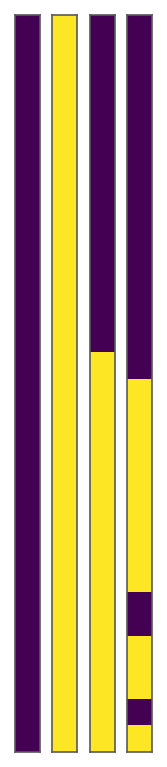
\includegraphics[height=1.8cm]{../../figures/darcy/darcy_input_boundary_strips.png}};
\node[font=\footnotesize, above=2pt of bnd_in] {$a|_{\partial\Omega}$};

% INTERIOR bottom branch
\node[inner sep=0pt] (int_in) at (2.6, -1.4)
    {
\includegraphics[width=1.8cm]{../../figures/darcy/darcy_input_interior.png}};
\node[font=\footnotesize, below=2pt of int_in] {Interior $a|_{\Omega^\circ}$};

% Split
\coordinate (split) at ($(input.east)+(0.3,0)$);
\draw (input.east) -- (split);
\draw[->] (split) |- (bnd_in.west);
\draw[->] (split) |- (int_in.west);
\fill (split) circle (1.5pt);

% ---- EXPANDED MLP BLOCK ----
\node[draw, rounded corners=3pt, fill=white,
      minimum width=3.8cm, minimum height=1.8cm] (mlp) at (5.0, 1.4) {};

\node[draw, rounded corners=2pt, fill=white,
      minimum width=1.0cm, minimum height=0.65cm,
      font=\footnotesize, align=center] (mlp_inner) at (3.85, 1.4) {MLP $\phi$};

\foreach \i/\shade in {0/20, 1/45, 2/30, 3/55} {
    \fill[violet!\shade] (5.01, 0.935+\i*0.25) rectangle (5.19, 1.115+\i*0.25);
    \draw[violet!65, thin] (5.01, 0.935+\i*0.25) rectangle (5.19, 1.115+\i*0.25);
}
\node[inner sep=0pt, minimum width=0.18cm, minimum height=0.93cm] (coeff) at (5.1, 1.4) {};
\node[font=\footnotesize, above=0.0pt of coeff] {$\mathbf{c}$};

\node[inner sep=0pt] (profile) at (6.1, 1.4)
    {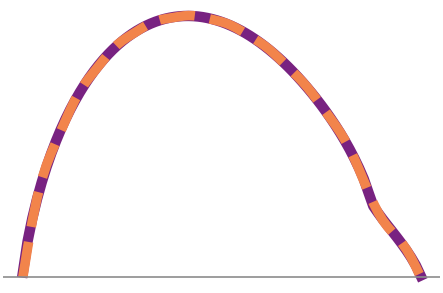
\includegraphics[width=1.1cm]{../../figures/darcy/darcy_sine_basis_right_boundary_diagram.png}};

\draw[->, thin] (mlp_inner.east) -- (coeff.west);
\draw[->, thin] (coeff.east) -- (profile.west);

\node[font=\small, above=4pt of mlp] {\textbf{Sine Constraint}};

% ---- TRANSFORMER ----
\node[netbox] (transformer) at (5.0, -1.4) {Transformer\\backbone $f$};

\draw[->] (bnd_in.east) -- (mlp.west);
\draw[->] (int_in.east) -- (transformer.west);

% OUTPUT BOUNDARY STRIPS
\node[inner sep=0pt] (bnd_out) at (7.4, 1.4)
    {
\includegraphics[height=1.8cm]{../../figures/darcy/darcy_output_boundary_strips.png}};
\node[font=\footnotesize, above=2pt of bnd_out] {$\hat{u}|_{\partial\Omega}$};

% OUTPUT INTERIOR
\node[inner sep=0pt] (int_out) at (7.4, -1.4)
    {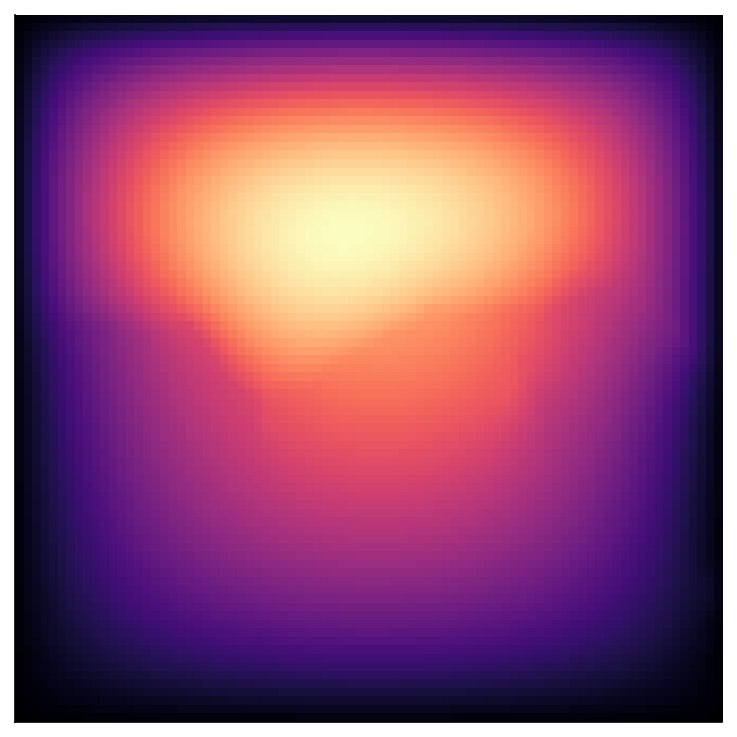
\includegraphics[width=1.8cm]{../../figures/darcy/darcy_output_interior.png}};
\node[font=\footnotesize, below=2pt of int_out] {Interior $\hat{u}|_{\Omega^\circ}$};

\draw[->] (mlp.east) -- (bnd_out.west);
\draw[->] (transformer.east) -- (int_out.west);

% FINAL OUTPUT
\node[inner sep=0pt] (output) at (10.1, 0)
    {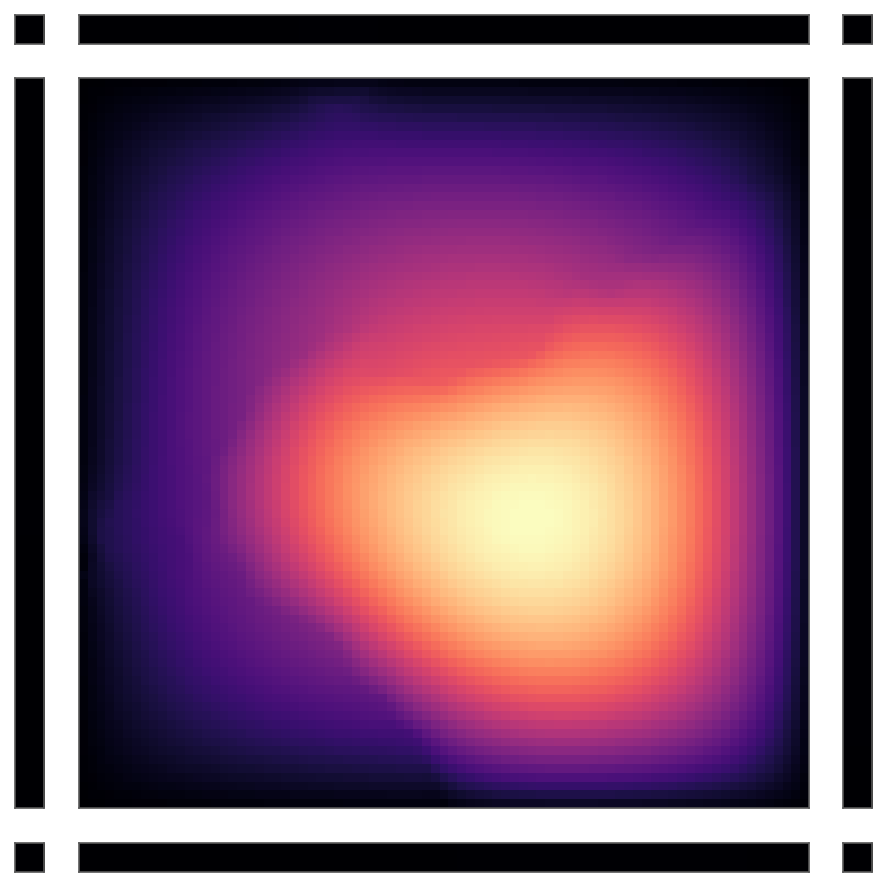
\includegraphics[width=1.8cm]{../../figures/darcy/darcy_output_boundary_decomposition.png}};
\node[font=\footnotesize, below=2pt of output] {Output $\hat{u}(\mathbf{x})$};

% Merge
\coordinate (merge) at ($(output.west)+(-0.3,0)$);
\draw (bnd_out.east) -- ++(0.3,0) |- (merge);
\draw (int_out.east) -- ++(0.3,0) |- (merge);
\draw[->] (merge) -- (output.west);
\fill (merge) circle (1.5pt);

\end{tikzpicture}
\end{document}
